
%% One page layout:
% Margins: left 40mm, rigt 25mm, top and bottom 25mm
% (latex adds extra 1in)
\documentclass[12pt,a4paper]{report}
\setlength\textwidth{145mm}
\setlength\textheight{247mm}
\setlength\oddsidemargin{15mm}
\setlength\evensidemargin{15mm}
\setlength\topmargin{0mm}
\setlength\headsep{0mm}
\setlength\headheight{0mm}
% \openright zařídí, aby následující text začínal na pravé straně knihy
\let\openright=\clearpage

%% Two pages layout:
% \documentclass[12pt,a4paper,twoside,openright]{report}
% \setlength\textwidth{145mm}
% \setlength\textheight{247mm}
% \setlength\oddsidemargin{15mm}
% \setlength\evensidemargin{0mm}
% \setlength\topmargin{0mm}
% \setlength\headsep{0mm}
% \setlength\headheight{0mm}
% \let\openright=\cleardoublepage

\usepackage[utf8]{inputenc}
\usepackage{graphicx}
\usepackage{amsthm}

\usepackage[unicode]{hyperref}   % Musí být za všemi ostatními balíčky
\hypersetup{pdftitle=Implementing control flow resolution in dynamic language}
\hypersetup{pdfauthor=Štěpán Šindelář}

%%% Small styling hacks

% Tato makra přesvědčují mírně ošklivým trikem LaTeX, aby hlavičky kapitol
% sázel příčetněji a nevynechával nad nimi spoustu místa. Směle ignorujte.
\makeatletter
\def\@makechapterhead#1{
  {\parindent \z@ \raggedright \normalfont
   \Huge\bfseries \thechapter. #1
   \par\nobreak
   \vskip 20\p@
}}
\def\@makeschapterhead#1{
  {\parindent \z@ \raggedright \normalfont
   \Huge\bfseries #1
   \par\nobreak
   \vskip 20\p@
}}
\makeatother

% Toto makro definuje kapitolu, která není očíslovaná, ale je uvedena v obsahu.
\def\chapwithtoc#1{
\chapter*{#1}
\addcontentsline{toc}{chapter}{#1}
}

\begin{document}

% Trochu volnější nastavení dělení slov, než je default.
\lefthyphenmin=2
\righthyphenmin=2

%%% Titulní strana práce

\pagestyle{empty}
\begin{center}

\large

Charles University in Prague

\medskip

Faculty of Mathematics and Physics

\vfill

{\bf\Large MASTER THESIS}

\vfill

\centerline{\mbox{
\includegraphics[width=60mm]{img/logo.pdf}}}

\vfill
\vspace{5mm}

{\LARGE Štěpán Šindelář}

\vspace{15mm}

% Název práce přesně podle zadání
{\LARGE\bfseries Implementing control flow resolution in dynamic language}

\vfill

% Název katedry nebo ústavu, kde byla práce oficiálně zadána
% (dle Organizační struktury MFF UK)
Department of Software Engineering of the Charles University in Prague

\vfill

\begin{tabular}{rl}

Supervisor of the master thesis: & Filip Zavoral, Ph.D. \\
\noalign{\vspace{2mm}}
Study programme: & Software Systems \\
\noalign{\vspace{2mm}}
Specialization: & specialization \\
\end{tabular}

\vfill

Prague 2014

\end{center}

\newpage

%%% Následuje vevázaný list -- kopie podepsaného "Zadání diplomové práce".
%%% Toto zadání NENÍ součástí elektronické verze práce, nescanovat.

%%% Na tomto místě mohou být napsána případná poděkování (vedoucímu práce,
%%% konzultantovi, tomu, kdo zapůjčil software, literaturu apod.)

\openright

\noindent
Dedication.

\newpage

%%% Strana s čestným prohlášením k diplomové práci

\vglue 0pt plus 1fill

\noindent
I declare that I carried out this master thesis independently, and only with the cited
sources, literature and other professional sources.

\medskip\noindent
I understand that my work relates to the rights and obligations under the Act No.
121/2000 Coll., the Copyright Act, as amended, in particular the fact that the Charles
University in Prague has the right to conclude a license agreement on the use of this
work as a school work pursuant to Section 60 paragraph 1 of the Copyright Act.

\vspace{10mm}

\hbox{\hbox to 0.5\hsize{%
In ........ date ............
\hss}\hbox to 0.5\hsize{%
signature of the author
\hss}}

\vspace{20mm}
\newpage

%%% Povinná informační strana diplomové práce

\vbox to 0.5\vsize{
\setlength\parindent{0mm}
\setlength\parskip{5mm}

Název práce:


Autor:
Bc. Štěpán Šindelář

Katedra:  
Katedra softwarového inženýrství Univerzity Karlovy

Vedoucí diplomové práce:
Filip Zavoral, Ph.D., TODO: pracoviště
% dle Organizační struktury MFF UK, případně plný název pracoviště mimo MFF UK

Abstrakt:
% abstrakt v rozsahu 80-200 slov; nejedná se však o opis zadání diplomové práce

Klíčová slova:
dynamické programovací jazyky, statická analýza, PHP, \mbox{Phalanger}, .NET

\vss}\nobreak\vbox to 0.49\vsize{
\setlength\parindent{0mm}
\setlength\parskip{5mm}

Title:
Implementing control flow resolution in dynamic language

Author:
Bc. Štěpán Šindelář

Department:
Department of Software Engineering of the Charles University in Prague

Supervisor:
Filip Zavoral, Ph.D., TODO: pracoviště

Abstract:
% abstrakt v rozsahu 80-200 slov v angličtině; nejedná se však o překlad
% zadání diplomové práce

Keywords:
dynamic programming languages, static analysis, PHP, \mbox{Phalanger}, .NET

\vss}

\newpage

%%% Strana s automaticky generovaným obsahem diplomové práce. U matematických
%%% prací je přípustné, aby seznam tabulek a zkratek, existují-li, byl umístěn
%%% na začátku práce, místo na jejím konci.

\openright
\pagestyle{plain}
\setcounter{page}{1}
\tableofcontents

%%% Jednotlivé kapitoly práce jsou pro přehlednost uloženy v samostatných souborech
\chapter{Introduction}

    \section{Problem Description}
    Static type analysis of a dynamic language, benefits: compiler optimizations, IDE support - bug hunting analysis.

    \section{Thesis structure}
%pygmentize_options: -O startinline=True

\chapter{Analysing PHP Code}

    The PHP programming language first appeared in 1995\cite{phphist}. Over the years 
    the language has evolved and so have the ways how programmers use it. 
    This project focuses on PHP version 5.5\footnote{From this point, 
    if the PHP version is not stated explicitly, it is implicitly 5.5.} 
    and the aim for the analysis 
    is to work well on PHP source code written in an object oriented style, 
    using modern PHP patterns and idioms that are described later in 
    this text. The analysis, however, should provide correct results for 
    any valid PHP code of any PHP version. We do not focus only on websites, but also on 
    PHP libraries and frameworks that by themselves do not contain 
    any PHP files that produce HTML or any other output for the user.
    
    \section{PHP semantics}
    This section describes some important parts of the semantics of 
    the PHP programming language, especially those that represent a 
    challenge for static analysis.
    
    \subparagraph*{}    
    In PHP, local or global variables, object fields and function or 
    method parameters are dynamically typed, which means that they 
    can hold values of completely different types at different 
    times of the execution.
    
    \subsection{Local Variables}
    Local variables in PHP do not need to be declared explicitly. 
    Instead the first usage of a variable is also its declaration. 
    If a variable's value is used before the variable got any 
    value assigned, then the interpreter generates a notice, 
    however the execution continues and value \code{null} is 
    used instead. A variable can get a value assigned to it when it 
    appears on a left hand side of an assignment or when a 
    reference to that variable is created, in which case it gets value 
    \code{null}, but no notice is generated. References are 
    discussed in one of the following subsections.

    The scope of a local variable is always its parent function not the 
    parent code block as in other languages like C or Java. 
    So in the following 
    example, the usage of variable \code{\$y} at the end 
    of the function can generate uninitialized variable notice, 
    however, if \code{\$x} was equal to \code{3}, 
    \code{\$y} will have a value although it 
    was declared in the nested code block.

%pygmentize_begin php
% function foo($x) {
%   if ($x == 3) { $y = 2; }
%   echo $y; // uninitialized variable if x != 3
% }
%pygmentize_end
    
    \subsection{Global and Local Scope}
    PHP distinguishes two scopes for variables: global scope and 
    local scope. Local scope is a scope of local variables 
    within a user defined routine.         
    Variables that are declared 
    in global scope, that is outside of a user defined routine, 
    are available anywhere in global scope and are called 
    global variables. Global variables are also available 
    in user defined routines as long as they are imported 
    into the routine's scope using the keyword \code{global}.
    
%pygmentize_begin php
% $g1 = 1;  // global variables g1 and g2
% $g2 = 2;
% function foo() {
%   global $g1;
%   echo $g1;   // prints the value of global variable g1
%   $g2 = 4;   // sets the value of local variable g2,
%   // because global variable g2 was not imported, 
%   // its value does not change
% }
%pygmentize_end

    Global variables can be imported and used in any user defined 
    routine. This means that even if we know some type information 
    about a global variable's value at some point in the analysed 
    code (e.g. straight after assignment to that variable), 
    any time another user defined routine is invoked, we 
    have to take into account that the other routine can 
    change the value of the global variable even if we do not 
    pass the global variable to the invoked routine 
    as an argument passed by reference.

    \subsection{Closures}
    PHP also supports anonymous functions. An anonymous function has its 
    own scope as any other function and its local variables are not visible 
    to the scope where it was declared. Variables from the parent 
    scope are available in the closure scope only if they are 
    explicitly imported to its scope and they can be captured 
    by value or by reference. Only the later represents a 
    challenge for the analysis, because any code that can 
    access the closure can invoke it and thus change the 
    values of variables imported to the closure's scope 
    by reference. By invoking a closure, we can influence 
    the values of variables in a completely different 
    and otherwise inaccessible scope.
    
    \subsection{References}
    References in PHP are similar, but not same, as pointers 
    in the C programming language. PHP has a special 
    operator \code{=\&} (assign by reference) that turns 
    the variable on the 
    left hand side into a reference to the 
    variable on right hand side. For example \code{\$a=\&\$b}, 
    after this, any assignment 
    to \code{\$a} will in fact change the 
    value of \code{\$b} and wherever 
    the value of \code{\$a} is used (e.g. in an expression), 
    the value of \code{\$b} is used instead.
    
    The variable where the reference is pointing to is determined 
    in a transitive fashion, which means that if we assign 
    by reference another reference, the new reference will 
    point to where the other reference was pointing to, 
    but the intermediate link is lost. The following example 
    illustrates this.
    
%pygmentize_begin php
% $a =& $b;       // a points to b
% $c =& $a;       // c points to where a points, that is b
% $a =& $d;       // a points to d, but c still points to b
%pygmentize_end    

    \subsection{Arrays}
    Arrays in PHP do not have to be homogenous and 
    they can be indexed by either integers or strings.
    In fact, PHP arrays are hash maps rather than arrays 
    in the usual sense and that is also how they are 
    implemented internally. 
    
    String indexed heterogenous arrays are often used 
    as flexible ad-hoc structured data type. 
    Instead of defining a class 
    with required fields, one can use what would be a 
    field name as an index into an array. Such arrays 
    are usually indexed only with finite number of 
    constant string values. 
    
    In this light, it is no 
    surprise that using the subscribe operator 
    \code{[]} with string index on an object instance will 
    access the field with the same name as the index value.

    \subsection{Interesting Control Flow Structures}
    The \code{break} and \code{continue} statements with 
    optional numeric argument are supported in PHP in a 
    similar way as in other standard imperative programming 
    languages. There are, however, important differences 
    to be noted.
    
    Firstly, The numeric argument can be an arbitrary 
    expression in some of the older versions of PHP, in which 
    case we cannot statically determine the target of 
    the jump for the control flow resolution.
    
    Secondly, the \code{switch} statement is considered 
    a loop for the purposes of both \code{break} and 
    \code{continue}. The semantics of \code{break} 
    is intuitive. One of the meaningful use cases is to 
    break a loop from within a \code{switch} by 
    using \code{break 2}. The semantics of 
    \code{continue} statement 
    is perhaps not so intuitive: within a \code{switch} 
    it works the same way as \code{break}.
    
    \subparagraph*{Switch Statement Semantics.} 
    The basic semantics of the \code{switch} statement in PHP is 
    again very similar to that of other standard imperative 
    programming languages. The \code{switch} statement in PHP 
    permits an arbitrary expression as the value to be used 
    for comparison with values of its \code{case} labels. Furthermore, 
    the values of \code{case} labels can also be arbitrary 
    expressions and because we are in a context of dynamic 
    programming language, they can again evaluate to a value 
    of any type.
    
    At runtime, the switch expression is evaluated only once 
    at the beginning, and if it has an undefined value (undefined variable, 
    void function call), then the control flow goes directly 
    to the default item, without evaluating the expressions 
    in the case items. If the value is defined, then it is 
    one by one compared to the values that the 
    \code{case} labels evaluate to. If a \code{case} label evaluates 
    to \code{boolean} value, then it is used to decide whether to 
    jump to that \code{case} item or continue with evaluating 
    the value of the next \code{case} label. Note that the value of 
    switch expression is not compared to the \code{case} label value. 
    If a \code{case} label evaluates to a complex type (\code{object} or \code{array}), 
    it is ignored and evaluation continues with the next \code{case} label. 
    And finally, if a \code{case} label evaluates to an 
    \code{integer}, \code{float} or \code{string} value, it is 
    compared to the switch expression. All these expressions can 
    have side effects due to usage of assignments as expressions 
    or calls of functions with side effects. 
    
    PHP also allows to place the \code{default} label anywhere in between 
    the other \code{case} labels. This can be used for fall-back 
    to or from a \code{case} item as in the following code sample 
    that is abbreviated version of actual code taken from the 
    WordPress\cite{wordpress} code base.
    
%pygmentize_begin php
%switch ( $status ) {
%    default:
%    case 'install':
%        $actions[] = '<a class="install-now" ...';
%        break;
%    case 'update_available':
%        $actions[] = '<a class="install-now" ...';
%        break;
%    case 'newer_installed':
%    case 'latest_installed':
%        $actions[] = '<span class="install-now" ...';
%        break;
%}
%pygmentize_end    
    
    
    \subsection{Conditional Declarations}
    User defined functions, classes, etc. are declared in 
    a global scope in PHP, that is a scope where one can 
    as well place any arbitrary code. Therefore a declaration 
    can be wrapped in any control structure. 
    It is not allowed to redeclare once declared symbol, however.
    
    A typical use case is to dynamically import a file 
    that may provide some functions and then check, 
    using \code{function\_exists}, whether the functions were 
    indeed declared and if not, provide default implementation.
    This is a pre-object-oriented way of doing overriding and 
    is usually not to be found in modern projects. Nonetheless, 
    WordPress still relies on this pattern in parts of its code base.
    
    Although the mentioned pattern could be deemed as 
    reasonable and useful. This feature allows 
    to write very problematic code as in the following example 
    that may or may not crash on fatal errors ``Cannot 
    redeclare foo()'' or ``Call to undefined function foo()'' 
    depending upon the user input.
    
%pygmentize_begin php
%while ($_POST['a'] != 3) {
%   function foo() { return 5; }
%   $_POST['a'] = $_POST['b'];
%}
%echo foo();
%pygmentize_end        
    
                
    \subsection{Auto-loading}
    Historically, in PHP in order to reference any symbol 
    from a different file, one had to import that 
    file explicitly. Newer versions of PHP support  
    customized auto-loading. A used defined routine 
    can be invoked by the runtime every time an 
    undefined class is referenced. 
    The auto-loading routine is then responsible for 
    importing the file(s) that contain the code of the 
    required class. 
    
    Auto-loading routine can use arbitrary logic to 
    determine what file(s) to import, in fact, it can 
    execute arbitrary code. Typical 
    pattern used for example in 
    Zend Framework\cite{zendframework} before namespaces were 
    introduced to PHP is to have a file per class and use 
    class names in form of 
    \code{CodeFolder1\_SubFolderName\_FileName} for 
    a class placed in file 
    \filepath{CodeFolder1\SubFolderName\FileName.php}.
    
    \subsection{PHPDoc Annotations}
    Although not part of the official PHP syntax, 
    there is a widely recognized format for documentation 
    comments of JavaDoc style called PHPDoc. PHPDoc comments 
    may contain type information that cannot be expressed using 
    PHP syntax. For example, PHP allows ``type hints'' 
    for routine parameters, but only for class types, 
    not for primitive types like \code{int}. However, 
    primitive type expectations can be included in the 
    documentation comments. The important difference 
    is that PHP will throw an exception at runtime if 
    a routine is invoked with a parameter of different 
    type than what its ``type hint'' is. The documentation
    comments, on the other hand, are of course ignored 
    by the runtime.
    
    The PHPDoc defines a fairly advanced syntax for expressing 
    type information. It supports multiple 
    primitive and class types, homogenous and heterogenous arrays as well 
    multidimensional arrays, and some constants like \code{false}.
    For example, in the following code the documentation 
    comment tells us that function \code{foo} can return 
    either \code{null}, or \code{false} (but should never 
    return \code{true}), or an array of \code{integer} values.
    
%pygmentize_begin php
% /**
%  * @return null|false|int[]
%  */
% function foo() { ...
%pygmentize_end
    
    \section{Static Code Analysis}       
        Static analysis of source code is an analysis that is performed without 
        executing the code. This means that we do not need to have a
        web server, for example, in order to analyse code of a web application. 
        We can also guarantee some properties of the analysis that would not 
        be possible to guarantee if we executed the code. Namely the halting property and 
        upper bounds on time and space complexity. Arbitrary code may not 
        halt if executed, but static analysis of such code can still halt 
        and give results.
        
        Static analysis can be used to get possible types of an expression in 
        a dynamically typed language, to find out expressions that have constant 
        value through constant propagation and many other problems. 
        Static analyses usually do not give accurate solution, but 
        its approximation, which can be an over-approximation or 
        an under-approximation and it is up to the designer and user of the analysis 
        which one is acceptable for his or her\footnote{``His'' or ``he'' 
        should be read as ``his or her'' or ``he or she'' through the rest of the text.} 
        purposes.

        Data Flow Analysis (DFA)\cite{aho1985compilers}, \cite{nielson1999principles} has 
        become a de-facto standard type of analysis for most of the optimizing compilers and 
        other more complex static analyses are either directly based on DFA or on 
        the ideas behind DFA. DFA is also used in Control Flow for Phalanger. 
        In the rest of this section, we provide brief description of 
        firstly DFA in general and then how we have leveraged DFA for 
        the purposes of PHP code analysis.
        
        %---------------------------------------------------------------------------------------
        \subsection{Program State}
        Execution of a program can be seen as a series of transformations of 
        the program state. Each individual program instruction, when executed, 
        can change the program state and produces its \emph{output state}.         
        How exactly is defined by the instruction's semantics and it typically 
        depends on the \emph{input state}, which is a program state produced 
        by the previously executed instruction. 
        
        The goal of a static analysis is to devise some useful piece of information 
        about how instruction $i$ can change the program state, so that it can 
        be used for program optimization or to reveal potentially problematic 
        instructions. For example, if assignment $a=4/b$ always assigns 
        constant value $1$ to $a$, because $b$ happens to be equal to $4$ 
        in any possible program state preceding $a=4/b$, we can change 
        $a=4/b$ to $a=1$, which has the same affect to the program state. 
        If we instead found out that $b$ is always equal to $0$, we would 
        know that this instruction will cause an exception.
        
        The result we expect from a static analysis is, for each instruction 
        in the program, provide some useful property of program state transformation 
        that always holds every time the instruction is executed. 
        The analyses differ in the properties they compute. 
        We will call such computed property a \emph{data-flow}.
        
        
        %---------------------------------------------------------------------------------------
        \subsection{Control Flow Graph.} 
        DFA is typically performed on a control flow graph, 
        although there exist approaches to DFA 
        without explicit control flow graph 
        construction \cite{mohnen2002graph}.
        
        Control flow graph nodes, also called basic blocks, 
        are program statements that are always executed sequentially. 
        Directed edges represent the control flow between basic blocks, 
        for example, jumps in the control flow due to conditionals, 
        \code{goto} statements or any other statements that can change 
        the flow of the program.        
        Control flow graphs usually contain two special nodes: 
        entry node and exit node. The entry node does not have any 
        incoming edges and all the paths lead to the exit node.        
        An example of a control flow graph is given in figure \ref{cfg}.
        
\begin{table}[h]
  \begin{tabular}{ l | m{6cm} }
  \centering
    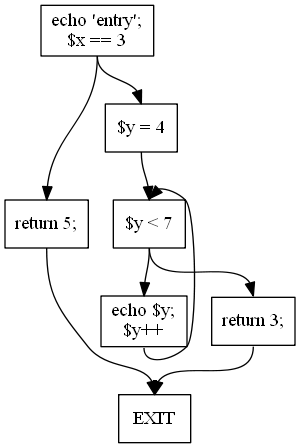
\includegraphics[scale=0.7]{img/cfg.png}
  &
 
\begin{minipage}{6cm}
%pygmentize_begin php
%   echo 'entry';
%   if ($x == 3)
%       $y = 4;
%   else
%       return 5;
%        
%   while ($y < 7) {
%       echo $y;
%       $y++;
%   }
%
%   return 3;
%pygmentize_end
\end{minipage}

  \\
  \end{tabular}
  \caption{Control flow graph\label{cfg}}  
\end{table}        
        
        %---------------------------------------------------------------------------------------
        \subsection{Transfer functions}
        
        We say that the input state of a statement is associated with 
        the \emph{program point before} the statement and the output state 
        is associated with the \emph{program point after} the statement. 
        Our aim is to calculate \emph{data-flow} value for both 
        program points for each statement, denoted $IN(s)$ and $OUT(s)$ for 
        a statement $s$.
        
        \subsubsection*{Single Statement}
        
        We can express the \emph{data-flow} for \emph{program point after} 
        a statement as a function of the \emph{data-flow} of 
        \emph{program point before} the statement, also called \emph{transfer function}. 
        Formally if $f_t$ is a \emph{transfer function}, then $f_t(IN(s))=OUT(s)$.
        Each type of statement will have a different \emph{transfer function} 
        that will reflect the semantics of the statement. 
        
        \emph{Transfer functions} are often described in the form of inference rules. 
        An example of an inference rule can be 
        ``if the types of expressions $e_1$ and $e_2$ are integers, then the type of 
        expression $e_1+e_2$ is integer''. Those rules can be more formally 
        described with the following notation        
        $$
        \infer{\vdash e_1+e_2 : Integer}{\vdash e_1 : Integer & \vdash e_2 : Integer}
        $$        
        where above the horizontal line we have hypothesis and below is 
        the conclusion. The exact notation is not important, we will be using it 
        intuitively to illustrate the ideas that we describe.
        
        \subsubsection*{Statements Interaction}
        
        The \emph{data-flow} for \emph{program point before} a statement 
        depends on the \emph{data-flow} of \emph{program point after} the 
        last executed statement. Let us consider a basic block $B$ with 
        statements $s_0, s_1, ..., s_n$.
        
        In the case of any $s_i \neq s_0$, that is any statement but 
        the first one, there is only one statement whose execution 
        can precede the execution of $s_i$ and that is the previous statement 
        in the sequence: $s_{i-1}$. So we have $IN(s_i) = OUT(s_{i-1})$ 
        for $i\in{[1..n]}$. 
        
        In fact, thanks to this property, we can define \emph{transfer function} 
        $f_B$ of a basic block as composition of transfer functions of 
        its statements. Formally: 
        
        \[ f_B = f_{s_n} \circ f_{s_{(n-1)}} \circ ... f_{s_0} \]
        
        where $f_{s_i}$ is the transfer function for statement $s_i$.            
        Furthermore, we denote \emph{data-flow values} of basic block as 
        $IN(B)=IN(s_1)$ and $OUT(B)=OUT(s_n)$. From the definitions we can 
        observe simple identities: 
        
        \[ f_B(IN(s_1))=f_B(IN(B))=OUT(B)=OUT(s_n) \]
        
        The first statement $s_1$ of the basic block has to be 
        handled differently. Its execution can be preceded by 
        execution of the last statement of any of 
        the basic blocks $B_1, B_2, ..., B_m$ that precede basic block 
        $B$ in the control flow graph. One of the possibilities to deal with 
        this, is to combine \emph{data-flows} $OUT(B_1), ..., OUT(B_m)$ into 
        single \emph{data-flow} that approximates all of them. 
        Nonetheless, the way the \emph{data-flows} are combined depends 
        on the concrete \emph{data-flow} type and thus 
        should be defined by the analysis. We denote the function to 
        combine \emph{data-flows} as $\mathit{MEET}$. 
        
        \subsubsection*{Equations for Data-Flow}
        
        If we put everything together, we get a set of equations:
        \begin{align*}
            OUT(B_i) &= f_{B_i}(IN(B_i)) \\
            IN(B_i) &= \mathit{MEET}(OUT(P_0), ..., OUT(P_m)) \\ 
        \end{align*}
        where $P_i$ is predecessor of $B_i$ in the control flow graph. 
        The analysis must also define value of $IN(START)$, that is 
        \emph{input state} for the initial node, which does not have 
        any predecessors.
        
        \subsubsection*{Example}
        We will illustrate the system of \emph{data-flow} equations on a 
        simple example. The subject of our analysis will be the 
        type of the variable \code{\$i} in the code sample in figure \ref{dfacfg}.
        
        \emph{Data-flow} will be a set of possible types of variable $i$ and 
        initial \emph{data-flow} of the start node will be an empty set.

\begin{table}[h]
  \begin{tabular}{ l | m{6cm} }
  \centering
    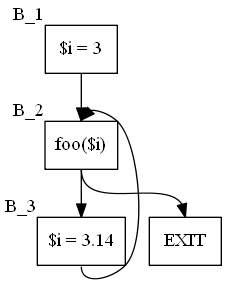
\includegraphics[scale=0.7]{img/dfa-cfg.png}
  &
 
\begin{minipage}{6cm}
%pygmentize_begin php
%   $i = 3;
%   while (foo($i)) {
%       $i = 3.14;
%   }
%   // exit
%pygmentize_end
\end{minipage}

  \\
  \end{tabular}
  \caption{Code for Data-Flow Example\label{dfacfg}}  
\end{table}

        \emph{Transfer functions}: we will assume that function call does 
        not change state, therefore the transfer function of 
        function call is identity -- $OUT(s)=IN(s)$. Assignment of 
        a constant \code{c} of type \code{T} to \code{\$i} changes 
        type of \code{\$i} to \code{T}.
        
        \emph{MEET} operation will be union of the sets of 
        possible types of \code{\$i}.
        
        The set of equations is in this case
        
        \begin{align*}
            OUT(B_1) &= f_{B_1}(IN(B_1))=f_B(\emptyset) \,\,\,\,\,\text{(initial node)} \\
            OUT(B_2) &= f_{B_2}(\mathit{MEET}(OUT(B_1), OUT(B_3))) \\
            OUT(B_3) &= f_{B_3}(OUT(B_2))     
        \end{align*}
        
        Knowing that $f_{B_1}$ and $f_{B_3}$ are constant functions, because 
        the assignment changes type of \code{\$i} to \code{T} without taking 
        the \emph{input data-flow} into account, and $f_{B_2}$ is identity 
        function, we can simplify the equations to

        \begin{align*}
            OUT(B_1) &= \left\{ \mathit{Integer} \right\} \\
            OUT(B_2) &= f_{B_2}(\mathit{MEET}(OUT(B_1), OUT(B_3))) \\
            OUT(B_3) &= \left\{ \mathit{Double} \right\} \\
            \\
            OUT(B_1) &= \left\{ \mathit{Integer} \right\} \\
            OUT(B_2) &= f_{B_2}( \left\{ \mathit{Integer} \right\} \cup \left\{ \mathit{Double} \right\} ) = 
                \left\{ \mathit{Integer}, \mathit{Double} \right\} \\
            OUT(B_3) &= \left\{ \mathit{Double} \right\}
        \end{align*}
        
        With this result we can, for example, check that function \code{foo} 
        is invoked with correct argument type, because from $IN(B_2)$ we 
        know that \code{\$i} at the moment of invocation of \code{foo} 
        can be either of type \code{Integer} or \code{Double}.
                
        \subsection{Finding Solution for the Data-flow Equations}
        
        \subsubsection*{Lattices.}
        The algorithm for finding a solution to a set of data-flow 
        equations is based on algebraic structures called lattices. 
        A lattice is a partially ordered set in which every 
        two elements have a least upper bound, called supremum, 
        and a greatest lower bound, called infimum.
        
        \emph{Bounded lattice} is a lattice that has 
        a greatest element and a least element, 
        usually denoted as $\top$ and $\bot$. 
        A bounded lattice is depicted in figure \ref{lattice}.       
        
\begin{figure}[h]  
  \centering
    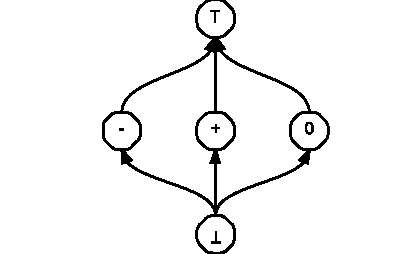
\includegraphics{img/lattice.pdf}
  \caption{Bounded lattice with 5 elements.\label{lattice}}    
\end{figure}

        There are several properties of lattices important for DFA.
        
        If we have a finite bounded lattice $(S, \leq_{s})$ and a function 
        $f:S\rightarrow{S}$ that is monotonous, in order words, 
        $\forall{a,b\in{S}}: a\leq_s{b} \Rightarrow f(a)\leq_s{f(b)}$, 
        then $\forall{x\in{S}}$ $\exists{k\in\mathbb{N}}$, such that 
        $f^k(x)=f^{(k+1)}(x)$. $f^k(x)$ is called a fixpoint.
        
        Intuitively, $f$ has to have a fixpoint because 
        for every argument $y$, it must either return 
        $y$ itself, but then $y$ is a fixpoint, or it 
        returns another element that is strictly 
        greater than $y$, but this cannot go on forever, because eventually 
        $f$ will be given $\top$ for which it does not have 
        any other option but returning $\top$ and we 
        have a fixpoint again.
        
        From this property further follows that if we use finite 
        lattice's elements as a domain for transfer functions, 
        and the transfer functions are monotonous, then the set of 
        data-flow equations has a solution, which is a safe 
        approximation of the, in a sense, best solution to the 
        data flow problem. Details can be found in \cite{kildall1973unified}.
        
        Product lattice obtained from two or more lattices 
        is also a lattice, which can simplify the design of 
        data flow analyses.        

        \subsubsection*{The Iterative Algorithm}
        
        The algorithm to find the solution to the data-flow equations 
        initially sets $OUT(B_i)$ for every basic block to the initial 
        \emph{data-flow}, which should be the lowest element of the lattice. 
        Then it iteratively takes a basic block $B_j$ such that 
        its input \emph{data-flow} $IN(B_j)$ has changed or is not 
        initialized yet and computes $OUT(B_j)$, which might change 
        the input \emph{data-flow} of the ancestors of $B_j$. 
        The process is repeated until a the system stabilizes. 
        
        The algorithm can take basic blocks in any order, however, 
        the reverse post order provides the best time complexity 
        \cite{aho1985compilers}.
        
        \subsubsection*{Bit Vectors as Data-flow Representation}

        The performance of the algorithm also depends on the implementation 
        of \emph{data-flow}, the $\textit{MEET}$ operations and the transfer 
        functions. 
        
        \emph{Data-flow} often represents a subset of a set of possible values 
        and the $\textit{MEET}$ operation is either union or intersection.
        For example, subset of all possible types of a variable. 
        Furthermore, we want to calculate the information for all 
        variables not only for one. If we know the number of variables $n$ and 
        types $m$ in advance, we can represent the \emph{data-flow} as 
        a bit-vector where groups of $m$ bits represent a data of 
        single variable and within those bits, value of bit with 
        index $i$ indicates whether the type with index $i$ is in the set. 
        Union or intersection can be implemented using fast bitwise operations.


        % -----------------------------------------------------------------------
        \subsection{Abstraction}
        \note{data-flow value for program point: an abstraction of the set of all possible program 
            states that can be observed for that point. Motivation for abstraction.}
            
        \note{TODO: convert the inference rules to rules with program state 
        and statement on the right side of the line.}
        
        Another example of problem that can be partly solved with static analysis 
        is the sign of integral variables. We can have inference rules of the 
        following form.
        $$
        \infer{\vdash v_1+v_2 : -7 (sign: \ominus)}
        {\vdash v_1 : -10 (sign: \ominus) & \vdash v_2 : 3 (sign: \oplus)}
        $$
        However, the implementation would not be very efficient and we sometimes 
        do not have the full information about variables values, but in some cases 
        we can deduce another less precise, but still useful piece of information 
        by other means. For example, variable of 
        type \code{unsigned integer} will always be positive, we can count on that 
        even if we do not know the actual value. What we 
        can do is to abstract the possible integral values with set 
        $\{0, \ominus, \oplus\}$ with the following meanings         
        \begin{itemize}
            \item $\ominus$ represents all negative integers,
            \item $\oplus$ represents all positive integers,
            \item $0$ represents zero,
        \end{itemize}                
        and rewrite the inference rules as follows:
        $$
        \infer{\vdash v_1+v_2 : \ominus}
        {\vdash v_1 : \ominus & \vdash v_2 : \ominus}
        $$
        Nonetheless, there is another problem. What to do when we have $\ominus$ 
        and $\oplus$ in the hypothesis.
        $$
        \infer{\vdash v_1+v_2 : ?}
        {\vdash v_1 : \ominus & \vdash v_2 : \oplus}
        $$
        The solution is to extend the domain so that it is closed under all operations. 
        We add another element to our set:
        \begin{itemize}
            \item $\top$ represents an unknown value (either positive, negative, or zero).
        \end{itemize}
        Then the rule will be:
        $$
        \infer{\vdash v_1+v_2 : \top}
        {\vdash v_1 : \ominus & \vdash v_2 : \oplus}
        $$
        And for example another rule dealing with $\top$ in hypothesis:
        $$
        \infer{\vdash v_1+v_2 : \top}
        {\vdash v_1 : \ominus & \vdash v_2 : \top}
        $$

        \note{Mention beta and gamma functions formalism for abstractions}
           

        % ----------------------------------------------------------------------
        \subsection{Intraprocedural Analysis}
        So far we have been discussing an analysis of a 
        single function or method\footnote{We will use term 
        routine to designate a global function, static or instance method}. 
        However, if we want to analyse whole program or 
        a library, the interaction between the routines 
        can be taken into account to make it more precise.
        
        \paragraph{Context Sensitive Intraprocedural Analysis.}
        The most precise solution would be to take into account 
        the calling context when analysing a function. 
        In different contexts, the function can be, 
        for example, given different parameters values 
        which may then influence the result of the analysis. 
        More precise result for a specific call site context 
        can be propagated to that call site, 
        yielding another gain in precision when 
        analysing the function that realises the call.
        
        \paragraph{TODO: Region Based Analysis.}
        
        \paragraph*{}
        \note{The following few paragraphs will discuss 
        feasibility of Context Sensitive Intraprocedural Analysis, 
        because call sites are not always known, 
        practical consequences and usual approaches to 
        make Context Sensitive Intraprocedural Analysis 
        more scalable.}
    
    % ----------------------------------------------------------------------------
    \section{Control Flow for Phalanger Approach}
        \note{Description of the analysis used in our case using the terminology 
        built up in the previous section. It will be more 
        abstract description, without technical details 
        about implementation.}
        
        \begin{itemize*}
            \item Modular approach that comes from assumption that 
                reasonably written PHP code will be close or equivalent to 
                statically typed code: (Aggressive Type Inference, by John Aycock: giving people 
                a dynamically-typed language does not mean that they write dynamically-typed programs.)
                \begin{itemize*}
                    \item No heap abstraction: we use classes -- enough for our purposes, no constant propagation, no null propagation, ...
                    \item No context sensitivity: we analyse routines in modular way.
                    \item Simple points-to analysis and lambda capture by ref.
                    \item Arrays: modelled as local variables.
                \end{itemize*}
        \end{itemize*}
        
\chapter{Existing Software}
    The aim was not to explore all the static analyzers, we chose Phantm to have a comparison...


    \section{Phantm\cite{kneuss2010using}}
    
    \section{HipHop Type Inference for Hack}
    
    \section{Weverca: Web Verification Tool\cite{hauzarhunting}}
\chapter{Implementation}

    \section{Implementation Specific Constraints}
    
    One of the requirements was that the project should be implemented 
    in the context of the Phalanger project. It should be ready 
    to be plugged in between the Phalanger's front-end and back-end and 
    it should also provide public interface useful for the 
    Phalanger PHP Visual Studio tools.
    
    \paragraph{Abstract Syntax Tree.} Phalanger front-end parses PHP code 
    into an Abstract Syntax Tree (AST) \cite{aho1985compilers} structure. 
    This structure is then traversed by the back-end using the 
    visitor design pattern \cite{gamma1994design}. Phalanger does not 
    use any other intermediate representation than AST and the 
    back end transforms the AST directly to Microsoft Intermediate Language (MSIL).
    
    In order to reduce the memory consumption and provide better 
    modularity, Phalanger code went through small architecture 
    refactoring before this project was started.     
    The classes representing the AST nodes originally contained 
    the code and data needed for emitting the corresponding 
    MSIL opcodes. This, however, represents 
    a coupling between the front-end and back-end and the 
    front-end cannot be used just on its own. In the new 
    version, the classes representing AST nodes are capable 
    of storing additional attributes in an extensible way 
    and the back-end have been rewritten to be an ordinary AST 
    visitor that uses the extensible AST nodes attributes.
    Additional attributes provide a way to annotate AST nodes 
    with any additional information, which in our case will be 
    the results of the analyses.    
    
    \paragraph{Integrated Development Environment Integration.}
    The PHP Tools for Visual Studio use Phalanger front-end in order to 
    parse PHP code into AST and then the AST is again traversed to provide 
    code completion and other features. All the AST nodes hold necessary 
    pieces of information, e.g. the position in the source file or 
    documentation comments.
    
    The aim of this project is to provide the results of type analysis 
    and other analyses to the integrated development environment so 
    that the possible errors and warnings can be visualised, e.g. underlined.
    
    The longer term aim of this project, not in the scope of this thesis, 
    is to replace the existing algorithms for code completion, 
    ``jump to definition'' and ``find usages'' features. Because 
    with a dynamic language like PHP, it is not trivial to 
    find all the usages of, for example, a class or determine 
    a definition of, for instance, a field accessed on some local variable. 
    In order to provide more precise results, 
    type analysis is needed.
    
    One of the challenging parts of integrated development 
    environment integration is also dealing with incomplete code 
    that is being typed in by the user. Therefore one of the requirements 
    was also that the analysis should be capable of 
    performing an ad-hoc re-analysis of once analysed 
    code with a new statement added. This ad-hoc re-analysis 
    should be, if possible, more effective that doing the 
    whole analysis again.
    
    \section{Overall Design}
    
    The project is divided into several modules.
    \begin{itemize}
        \item Control Flow Graph,
        \item Intermediate Representation of PHP Code (Phil, RPhil),
        \item Generic Data Flow Analysis Framework, 
        \item Tables with Type and Other Information, 
        \item Concrete Analyses:
        \begin{itemize}
            \item Dead Code Elimination, 
            \item Aliasing Analysis, 
            \item Constant Propagation,
            \item Type Analysis.
        \end{itemize}
    \end{itemize}
    
    The interactions between those modules on a conceptual level 
    when performing an analysis are depicted in diagram \ref{overalldiagram}. 
    Green elements represent extension points. Red arrows represent the 
    core flow of the algorithm.
    
\begin{figure}[h]  
  \centering
    \includegraphics*[width=\textwidth,height=\textheight,keepaspectratio,viewport=0 55 532 590]{img/ControlFlowModules.pdf}  
    \caption{Control Flow for Phalanger Design Overview\label{overalldiagram}}
\end{figure}    

    \subparagraph*{Intermediate Language.}
    One of the goals of the design was to stay as close as possible 
    to the original AST representation, so that the results of the 
    analysis can be easily propagated to an IDE and that the 
    Phalanger back-end does not have to be rewritten in order to 
    leverage the this project.
    
    Control Flow for Phalanger uses two intermediate representations 
    on a conceptual level, however, they are usually not explicitly 
    constructed as described later in the text. The purpose of the 
    intermediate representations is to simplify the design of the 
    analyses.
    
    \emph{Phil} stands for \emph{PHP Intermediate Language} and is very abstract 
    representations close to the original AST. Phil contains 
    only statements and expressions that can be in a Basic Block, 
    therefore it does not contain most of the control flow 
    changing statements like if, switch, or loops. 
    A Phil statement represents the smallest single step 
    of an execution that can change state of variables 
    or global state or throw an exception. Syntactic 
    constructs like \code{\$i++} are unfolded to 
    \code{\$i = \$i + 1}, which is then split to 
    evaluation of binary expression and assignment expression 
    that uses the result of the binary expression. In some sense, 
    Phil can be viewed as a three address code.
    
    \emph{RPhil} stands for \emph{Resolved PHP Intermediate Language}. 
    RPhil is basically a Phil with resolved symbols where possible. 
    By resolved symbols, we mean references to the elements 
    of Type Tables discussed in one of the following paragraphs. 
    In order to resolve the symbols, the module building RPhil 
    can use names explicitly expressed in the code, for example, 
    for direct local variable access \code{\$a}, or the results of 
    an analysis, for instance, the results of type analysis to 
    resolve method calls and fields references. 
    RPhil itself is typically consumed by the analyses, 
    so the accuracy of RPhil and subsequently of the 
    analyses results can be improved by iterative execution 
    of the analyses.
    
    \subparagraph*{Analyses.}
    The Data Flow Analysis is performed on Control Flow Graph 
    nodes called basic blocks. Each basic block contains 
    a list of Abstract Syntax Tree elements. This list is 
    then, usually on the fly, transformed to corresponding PHP 
    Intermediate Language elements before its elements are given 
    to the flow function of a concrete Data Flow Analysis 
    implementation. 
    
    Basic block can also contain already transformed PHP 
    Intermediate Language elements. However, the interface 
    does not change from the point of view of a concrete 
    Data Flow Analysis implementation.
    
    The Control Flow for Phalanger also contains and allows to 
    plug-in simple analyses that are performed for all 
    basic blocks sequentially without taking the control 
    flow into account. Each basic block is then analysed 
    only once. An example of such analysis is Aliasing Analysis.
    
    The last analysis type, which stands aside, is Dead Code 
    Elimination. It is performed on the Control Flow Graph, 
    but traverses it on its own as opposed to a concrete 
    Data Flow Analysis that only visits basic blocks 
    in order determined by the Data Flow Framework, 
    i.e. does not perform the graph traversal 
    on its own. Control Flow for Phalanger also allows 
    to add custom analyses that are performed on the raw 
    Control Flow Graph.
    
    \subparagraph*{Analyses Results.}
    The results of an analysis can be annotations added 
    to the AST node objects, or annotations of basic blocks, 
    which support extensible attributes in the same way as 
    AST nodes.
    
    The results of an analysis can also be pushed into 
    the Code Tables. Code Tables gather relevant information 
    about code elements like classes, functions, etc. 
    It is mainly type related information, 
    for example, a return type of a function, 
    but also which parameters are passed by reference or 
    whether the function returns a reference.
    
    \subparagraph*{Type Tables.} This module provides 
    almost the same information about routines, types, 
    global variables and constants as Code Tables. 
    However, in this case the information 
    is abstract, because it might not be directly related 
    to an actual element that can be found in the source code. 
    This is the case of library functions and classes, 
    but it also gives a possibility to merge the information 
    of two or more conditionally declared elements. 
    
    Although this kind of support for conditional declarations 
    has not been implemented, the design is prepared for it, 
    shall it be considered an important feature in the future. 
    At the moment, if two or more declarations are found, 
    the Type Tables behave as if they did not know the 
    element at all, which preserves correctness for the 
    price of loosing precision.
    
    \subparagraph*{Extensibility.}
    The whole project is designed as a class library and 
    framework with many extension points. Some of the 
    functionality can be used independently. For example, 
    Control Flow Graph builder to generate diagrams.
    
    Nonetheless, in order to provide better usability, 
    Control Flow for Phalanger also contains 
    a Facade class \code{AnalysisDriver} 
    that plugs in together all the necessary objects 
    and provides a simple interface to perform a defined 
    analysis of a file or a given piece of code.
    
    \section{The Intermediate Language}    
        \note{The aim of the intermediate representation is... 
        The three address code can be built by traversing the AST in 
        the order of execution... Some AST elements represent more 
        than one execution step...}
        
        \note{RPhil: the symbols are resolved using defined AST 
        nodes annotations for constant values and type information...
        \code{VarLikeConstructInfo} abstracts variables accesses...}
    
    \section{Control Flow Graph}
        \note{Description of the Control Flow graph construction}.
        
    \section{Data Flow Analysis}
        \note{Architecture of the generic algorithm implementation 
            using generics in C\# in a way that the graph the analysis 
            can be performed upon an arbitrary graph (not only CFG), 
            which can be useful if in the future some of the analyses 
            will be performed, for example, on a definition-use graph.}
        
    \section{Tables}
        \note{Intra-procedural dependencies handling \code{DependencyResolver}.}
    
    \section{Analyses}
        \subsection{Dead Code Elimination}
        \subsection{Aliasing Analysis}        
        \subsection{Constant Propagation}

    \section{Type Analysis}
        \note{
        \begin{itemize}
            \item Type Information representation
            \item Data Flow representation
            \item AST annotations
        \end{itemize}}

    \section{The Analyser pipeline and AnalysisDriver}
        \note{Description of the high level public interface 
        and the phases of the full analysis process.}
%pygmentize_options: -O startinline=True
\chapter{Results}
We evaluated Control Flow for Phalanger on several open source PHP projects. 
In order to have a comparison to another established tool of similar type, 
we analysed one of the PHP projects with both Control Flow for Phalanger and 
Phantm. The discussion of the differences in results is provided in the 
following section. The rest of the PHP projects were analysed only with 
Control Flow for Phalanger and the reported problems were manually inspected 
and categorized.


\section{Comparison to Phantm\label{phantmresults}}

The project we chose for comparison evaluation is Zebra\_Image \cite{zebraimage}. 
It is a PHP image manipulation library that consists of 1707 lines of code 
in one file and one class. Zebra\_Image code contains some type documentation, 
but incomplete and often written in a way that does not follow the standard 
PHPDoc type description grammar.

All the problems reported by either tool were briefly inspected and 
categorized. The results are presented in the following table and 
are very different for each tool, which can be due to the 
different approaches to the analysis. The actual problems reported and 
the possible reasons for the difference in results are discussed in 
the following paragraphs.

\begin{center}
    \begin{tabular}{| p{6cm} | r | r |}
    \hline
    \textbf{Category}           &   \textbf{Phantm}      &   \textbf{Control Flow for Phalanger} \\ \hline
    All Reported problems       &     130                &    1   \\ \hline
    Uninitialized variable use  &       2                &    1   \\ \hline
    Zebra\_Image dynamic fields  &       82               &    0     \\ \hline
    Any is not of type X        &       13               &    0     \\ \hline    
    Prototype errors            &       9                &    0     \\ \hline    
    Conversion: double to integer&       2               &    0     \\ \hline    
    Other type conversions      &       2               &    0     \\ \hline    
    Not categorized             &       17               &    0     \\ \hline    
    \end{tabular}
\end{center}

\subsubsection*{Reported Problems}

The uninitialized variable error appears to be genuine problem that would 
generate a notice at runtime. It was discovered by both tools. Because the 
variable in question is accessed as an array using the \code{[]} operator, 
Phantm reported it twice.

All the prototype errors are false positives probably due to the fact 
that Phantm does not distinguish mandatory and optional parameters. 
In PHP, any routine can take any number of arguments. Arguments explicitly 
named in the signature are mandatory, but any number of optional arguments can be 
accessed using intrinsic functions. Therefore it is not necessarily a prototype 
error if a routine is given more parameters than the number of 
parameters explicitly named in its signature.

PHP allows to use undeclared object fields, they are dynamically created when 
first used, usually assigned to. Zebra\_Image relies on this and dynamically 
creates some fields in certain methods and then uses them in 
other methods, which is reported by Phantm. Using fields without 
explicitly declaring them can be seen as a style error, especially in case 
of Zebra\_Image, because all the fields in question are in fact known 
beforehand and therefore it is perfectly possible to explicitly declare them. 
In other cases, however, this language feature enables useful patterns 
mainly in combination with magic \code{\_\_set} and \code{\_\_get} methods, as 
for example in model classes of Doctrine Object-Relational Mapper \cite{doctrine}.

Phantm regards some implicit type conversions as errors. Namely anything to 
string type conversion, which is typically used in PHP, and double to 
integer, which is more debatable, but nonetheless often used deliberately 
instead of cast or floor or ceiling functions.

\subsubsection*{Conclusion}

Those results can indicate that, although at first sight the aims of the
two tools are the same, under closer inspection, they differ. 
Phantm attempts to perform very precise analysis. For example, 
by modelling heap memory. Such precision is, in theory, more powerful 
and can discover more actual problems; yet, it also yields
many false positives. It would be possible to filter out the 
``likely to be'' false positives, but that would filter out those 
cases where due to the better precision, Phantm discovered 
actual error.

On the other hand, although being less precise, Control Flow for 
Phalanger seems to have better ratio of false positives. 
This could make it more suitable option for a day to day development, 
which is what it was in fact focused on. 

Due to this difference, the results for other PHP projects were 
manually inspected only in the case of Control Flow for Phalanger.


\section{Evaluation on open source PHP code}

For further evaluation, the following open source PHP frameworks and 
websites were chosen:

\begin{description}
    \item[PHPUnit:] a port of JUnit unit testing framework for PHP; it is a mature 
    and well established project that has been developed for more than 6 years 
    by 156 contributors. Being a unit testing framework, PHPUnit itself has extensive 
    unit test suite. For the experiment the master branch of the clone of the 
    repository retrieved on 18.5.2014 has been used. 
    
    \item[Nette:] popular general purpose PHP framework with long development 
    history and contributions from 137 developers. Nette has unit test suite 
    with good code coverage and the source code is very well documented including 
    the type documentation comments.
\end{description}

    \begin{comment}
    \item[Zend Framework:] popular general purpose PHP framework. Lorem ipsum...
        \note{over 3000 problems reported. Quite a big bite to chew with analysing and categorizing all of them.}        
        
    \item[Piwik:] open source version of Google Analytics. \note{few hundred problems found, not categorized yet}
    
    \item[PrestaShop:] open source e-commerce solution. \note{few hundred problems found, not categorized yet}
    
    \item[Composer:] popular dependency management system for PHP libraries. \note{few hundred problems found, not categorized yet}
    \end{comment}

An evaluation always started with downloading a git repository with the 
latest source code of given PHP project. Then the analysis was run and 
all the discovered problems were collected and categorized.
Actual errors were rectified and recorded as commits in the 
git repository. 

Often one real issue in the source code caused several 
warnings to be reported by the tool. For instance, if a documentation 
of a type of a field was not correct, most the lines where 
a value was assigned to that field were reported, however, the 
root of the cause was actually the only one line with the 
wrong type documentation. Such cases were counted as a 
single problem.

\subsection{Problems Taxonomy}

The problems were divided into few main categories 
described below.

\paragraph*{Style:} a category of problems that 
are not directly affecting the functionality of the 
application, but they can be considered as a bad 
coding style. 

\begin{itemize}
    \item[] \textit{Relaying on default return value} -- when an execution of a 
        routine does not end with a return statement, its 
        return value is \code{NULL} by default, which can then 
        be cast to values of other types, like \code{false} 
        for example. Developers rely on this feature and omit 
        the return statement if they want to return \code{NULL} or 
        something that \code{NULL} can be cast to.
\end{itemize}

\paragraph*{Documentation:} inconsistency of the PHPDoc type 
documentation and what the the code does. This category includes 
only cases where it is clear that the documentation is wrong, not the code, 
for example, due to updates in the code that were not reflected 
in the documentation. The inconsistency may also indicate 
another problem, in which case it does not belong to this category. 

Interestingly, most of the inconsistencies of type of a parameter 
of a function call typically lead through several routines that 
only forward the parameter to the next routine until 
eventually the routine that has a wrong documentation is reached.

\begin{itemize}
    \item[] \textit{Missing} \code{false} \textit{in return value type documentation} -- 
        this is common pattern in PHP where a routine returns \code{false} 
        when it fails to do what it was supposed to do. For example, 
        function \code{fopen} returns \code{resource} of \code{false} 
        if the resource could not be opened. It is so common that 
        developers tend to forget to put \code{false} into the documentation.
\end{itemize}

\paragraph*{Actual Error:} includes all problems that can cause 
an unexpected exception or unexpected runtime error or notice.


\paragraph*{False Positive:} problems reported by the tool that 
are not in fact real problems. Includes only false positives 
that cannot be eliminated because of fundamental design reasons 
or are not intended to be eliminated, because it would 
cause some actual positives to be missed.


\begin{itemize}
    \item[] \textit{Unused routine arguments} -- when a method is an override of 
        some base method, it can have the same signature and if some of the 
        parameters are not used, they are not reported. There are however 
        some cases where the routine is implementing some interface by convention 
        that is not explicitly expressed in the syntax of PHP.
        For example, the pre-object-oriented pattern for global functions 
        overriding. In such case the analyzer cannot determine that the unused 
        parameter is in fact a part of an interface. Note that such function 
        could omit the unused parameter and everything would work the same, 
        therefore this may or may not be considered a false positive.
    \item[] \textit{Amendable false positive} -- false positives 
        that are reported, although the algorithm the analyzer 
        is using should not report them. Those indicate errors 
        in the implementation.
    \item[] \textit{Built-in documentation errors} -- false positives 
        due to the inaccuracy of the documentation of built-in 
        functions and classes that was used in the experiment.
\end{itemize}

\subsection{Summary}

The following table provides a summary of the problems found. 
There is a table that lists concrete problems found PHPUnit 
available in appendix.

\newcommand{\subcat}[1]{\hspace{0.5cm}\small{\textit{#1}}} 
\newcommand{\reldefret}{\subcat{default return value}}

\newcommand{\sumh}[1]{\textbf{#1}}
%\newcommand{\sumh}[1]{\begin{turn}{60}#1\end{turn}}

\begin{center}
    \begin{tabular}{| p{5cm} | r | r | r | r | r |}
    \hline
    \sumh{Category}         &   \sumh{PHPUnit}      &   \sumh{Nette}    &   \sumh{total}   \\ \hline
    Style                   &   6                   &   0              &   6       \\ \hline
    \reldefret              &   2                   &   0              &   2       \\ \hline        
    Documentation           &   10                  &   1              &   11      \\ \hline    
    \subcat{missing false}  &   3                   &   0              &   3       \\ \hline
    Actual Error            &   1                   &   0              &   1      \\ \hline    
    False positive          &   8                   &   0              &   8      \\ \hline    
   \subcat{unused arguments}&   1                   &   0              &   1      \\ \hline        
    \subcat{amendable}      &   4                   &   0              &   4      \\ \hline            
 \subcat{built-in doc error}&   3                   &   0              &   3      \\ \hline
    \textbf{Total} 
    (excl. false positives) &17                   &   1              &   17      \\ \hline
    \end{tabular}
\end{center}



\subsection{Selected Problems}

\subsubsection*{Actual Error When Handling \code{DOMElements}}

The error is related to the following code (shortened).

%pygmentize_begin php
% function assertEqualXMLStructure(
%   DOMElement $expectedElement/*, ...*/) {
%   ///...
%   PHPUnit_Util_XML::removeCharacterDataNodes($expectedElement);
%   PHPUnit_Util_XML::removeCharacterDataNodes($actualElement);
%   //...
%   for ($i = 0; $i < $expectedElement->childNodes->length; $i++) {
%       self::assertEqualXMLStructure(
%           $expectedElement->childNodes->item($i) /*<<< error */
%           /*...*/);
% }
%pygmentize_end

The method \code{assertEqualXMLStructure} accepts only instances 
of \code{DOMElement}, but it invokes itself recursively with first 
argument of type \code{DOMNode}. Because according to the 
PHP documentation the value of the \code{childNodes} property 
of interface \code{DOMNode} is an instance of \code{DOMNodeList} 
and the method \code{item(integer)} of \code{DOMNodeList} 
returns \code{DOMNode}, it is a type mismatch error as \code{DOMNode} 
is not subtype of \code{DOMElement}.

In the PHP implementation of DOM model, the only implementations of 
\code{DOMNode} either inherit from \code{DOMElement} or 
implement \code{DOMCharacterData}, and those are removed 
from the \code{childNodes} collection by \code{removeCharacterDataNodes}. 
Therefore, in most cases, this code behaves as expected. 

However, the \code{DOMNode} interface can be implemented by any user 
defined class, which does not have to inherit from 
\code{DOMElement}, and if an instance of such class was present 
in the \code{childNodes} collection, the code would cause an 
exception when trying to invoke \code{assertEqualXMLStructure} 
with an argument of wrong type.

Note that if method \code{removeCharacterDataNodes} removed 
all the child nodes that are not instances of \code{DOMElement}, 
the code would be correct, but the error would still be reported, 
therefore it would be false positive.



\chapter{Conclusion}

    In this thesis we presented a project with code name 
    Control Flow for Phalanger, which can analyse PHP 
    source code in order to discover type related errors 
    and mismatches with type documentation.
    
    The Control Flow for Phalanger was evaluated on 
    three real world PHP project. Although, the tool 
    does not use heap abstraction and 
    does not perform context sensitive analysis, it was 
    still capable of discovering several real 
    issues with a good ratio of false positives. 
    
    This result may indicate that, were some imprecision 
    in the analysis results can be tolerated, the 
    modular approach we used can give results comparable 
    to those of tools that use more complex methods, with 
    possibly better scalability.

    \section{Future Work}
    
        \subsubsection*{Phalanger Integration}
        The Control Flow for Phalanger has not yet been fully 
        integrated into the Phalanger project. This includes 
        integration with the compiler in order to enable 
        code optimizations and evaluation of the possible 
        performance gain when running PHP websites like WordPress.
        
        \subsubsection*{Arrays Support}
        Array support has not been implemented yet. Variables 
        that can be of type array are analysed properly, but 
        the structure of the array is not analysed. Therefore 
        any time an element of an array is accessed, we do not 
        have any type information for it and have to assume 
        the worst -- it can be any type.
        
        Arrays in PHP are often used as ad-hoc structural 
        types like records in Pascal or structs in C. 
        In such case, the array is typically subscribed to 
        only by a set of known string constants, 
        which represents a good opportunity for 
        static analysis.
        
        One of the possible concepts for local arrays 
        analysis we would like to investigate further 
        is based on the fact that arrays in PHP have 
        copy semantics as opposed to most of the other 
        programming languages. We can model each constant 
        index of an array as a separate local variable. 
        For example, for code \code{\$a['x']=3} we create 
        two local variables: \code{\$a} and \code{\$a@x} 
        and the type of \code{\$a} would be an array and 
        the type of \code{\$a@x} would be an integer. 
        Such representation would still permit us to use 
        bit-vectors as the \emph{data-flow} representation.
        
        \subsubsection*{Performance Evaluation and Tuning}
        Some of the design decisions in Control Flow for 
        Phalanger were made for performance reasons. The 
        design is done an a way that permits further 
        performance targeted improvements, but first 
        an evaluation of the current performance is 
        required.
        
        One of the possible enhancements is more efficient 
        type information representation. Type information 
        is represented using a 64 bit value, however, 
        we can go even further and represent the type 
        information with 8 bit number, which will be an index 
        into a table with all the possible type information 
        instances for one routine. This would give us 255 
        possible combinations of types, which we assume is 
        enough for most of the routines. Since every expression 
        node in AST is annotated with type information and 
        \emph{data-flow} values are arrays of 
        type information, we expect memory consumption 
        and possibly performance improvement.
        
        %\subsubsection*{Context-sensitive Analysis}
        


%%% Seznam použité literatury
\def\bibname{Bibliography}
\addcontentsline{toc}{chapter}{\bibname}
\bibliographystyle{ieeetr}
\bibliography{bibliography}

%%% Tabulky v diplomové práci, existují-li.
\chapwithtoc{List of Tables}

%%% Přílohy k diplomové práci, existují-li (různé dodatky jako výpisy programů,
%%% diagramy apod.). Každá příloha musí být alespoň jednou odkazována z vlastního
%%% textu práce. Přílohy se číslují.
\chapwithtoc{Attachments}

\openright
\end{document}
